\documentclass[a4paper,11pt]{article}
\usepackage{amssymb, enumitem}

\parindent 0cm
\usepackage{amssymb,amsmath,amsthm,latexsym,epsfig,euscript,multicol}
\usepackage[utf8x]{inputenc}
\usepackage{listings,xcolor,bm}


\definecolor{mygreen}{rgb}{0,0.6,0}
\definecolor{mygray}{rgb}{0.5,0.5,0.5}
\definecolor{mymauve}{rgb}{0.58,0,0.82}
\lstset{
  backgroundcolor=\color{white},   % choose the background color; you must add
  basicstyle=\small\ttfamily,               % the size of the fonts that are used for the code
  breakatwhitespace=false,         % sets if automatic breaks should only happen at whitespace
  breaklines=true,                 % sets automatic line breaking
  captionpos=b,                    % sets the caption-position to bottom
  commentstyle=\color{mygreen},    % comment style
  deletekeywords={...},            % if you want to delete keywords from the given language
  escapeinside={\%*}{*)},          % if you want to add LaTeX within your code
  extendedchars=true,              % lets you use non-ASCII characters; for 8-bits encodings only, does not work with UTF-8
  firstnumber=1,                % start line enumeration with line 1000
  frame=single,	                   % adds a frame around the code
  keepspaces=true,                 % keeps spaces in text, useful for keeping indentation of code (possibly needs columns=flexible)
  keywordstyle=\color{blue},       % keyword style
  language=Python,                 % the language of the code
  morekeywords={*,...},            % if you want to add more keywords to the set
  numbers=left,                    % where to put the line-numbers; possible values are (none, left, right)
  numbersep=5pt,                   % how far the line-numbers are from the code
  numberstyle=\tiny\color{mygray}, % the style that is used for the line-numbers
  rulecolor=\color{black},         % if not set, the frame-color may be changed on line-breaks within not-black text (e.g. comments (green here))
  showspaces=false,                % show spaces everywhere adding particular underscores; it overrides 'showstringspaces'
  showstringspaces=false,          % underline spaces within strings only
  showtabs=false,                  % show tabs within strings adding particular underscores
  stepnumber=5,                    % the step between two line-numbers. If it's 1, each line will be numbered
  stringstyle=\color{mymauve},     % string literal style
  tabsize=4,	                   % sets default tabsize to 2 spaces
  title=\lstname                   % show the filename of files included with \lstinputlisting; also try caption instead of title
}
% Caracteres especiales
\def\A{\mathbb{A}}
\def\C{\mathbb{C}}
\def \N{\mathbb{N}}
\def \P{\mathbb{P}}
\def \Q{\mathbb{Q}}
\def \R{\mathbb{R}}
\def \Z{\mathbb{Z}}
\def \sen{\textrm{sen}}

\def\Np{$\N$}
\def\Zp{$\Z$}
\def\Qp{$\Q$}
\def\Rp{$\R$}
\def\Cp{$\C$}

\def\bb{\bm{b}}
\def\bu{\bm{u}}
\def\bv{\bm{v}}
\def\bx{\bm{x}}
\def\bA{\bm{A}}
\def\bB{\bm{B}}
\def\bD{\bm{D}}
\def\bE{\bm{E}}
\def\bM{\bm{M}}
\def\bT{\bm{T}}


\def\K{\textrm{K}}
\def\V{\textrm{V}}
\def\S{\textrm{S}}

\def\degres{$^\circ$}

\newcount\todno
\def\no{\global\advance\todno by 1 \the\todno}

\topmargin-2cm \vsize 29.5cm \hsize 21cm
\setlength{\textwidth}{16.75cm}\setlength{\textheight}{23.5cm}
\setlength{\oddsidemargin}{0.0cm}
\setlength{\evensidemargin}{0.0cm}


\theoremstyle{definition}
\newtheorem{ejer}{Ejercicio}
\newcommand{\bej}{\begin{ejer}}
\newcommand{\fej}{\end{ejer}}

\begin{document}

\centerline{{\small Universidad de Buenos Aires - Facultad de Ciencias Exactas y Naturales - Ciencias de Datos}}

\vskip 0.2cm

\hrule

\vskip 0.2cm

 \centerline{{\bf\Large{\sc Laboratorio de Datos}}}

 \vskip 0.2cm

 \centerline{\ttfamily Primer Cuatrimestre 2024}

\vskip 0.2cm

 \hrule

 \bigskip
 \centerline{\bf Práctica N$^\circ$ 2: Estad\'istica descriptiva y visualizaci\'on de datos.}
 \bigskip


\textbf{\bf Data frames}

Un data frame es una representaci\'on de los datos en formato de tabla en la que cada columna son vectores del mismo tamaño. Como cada columna es un vector, cada columna puede contener datos de un \'unico tipo. Se pueden pensar como variables.

\begin{enumerate}
\item Una forma de crear un data frame es utilizando un ``diccionario''. Todas las variables del diccionario deben ser vectores o listas de la misma longitud. Ejecutar el siguiente c\'odigo.

\begin{lstlisting}
data = {"nombre": ["Rodrigo", "Sergio", "Cristina", "Diana"], "altura": np.array([178, 172, 175, 168]), "peso": np.array([81.2, 76.1, 68.5, 64.0])}
display(data)

pacientes = pd.DataFrame(data)
display(pacientes)
\end{lstlisting}

\item ?`Cuál es la clase del objeto \lstinline{pacientes}? ?`Cuál es la clase de cada uno de los vectores columna? (para saber la clase de un objeto, utilizar el comando \lstinline{type}, para saber el tipo de datos de un array de numpy, utilizar \lstinline{np.dtype})

\item Guardar en una variable nueva el vector columna \lstinline{altura}. Pueden utilizar \lstinline{pacientes["altura"]} o \lstinline{pacientes.altura} (la primera opci\'on es preferible, la segunda puede dar error si el nombre coincide con alguna funci\'on ya existente).

\item Cargar la biblioteca \lstinline{gapminder} utilizando
\begin{lstlisting}
from gapminder import gapminder
\end{lstlisting}

Si da error es posible que no est\'e instalado. En tal caso ejecuten primero
\begin{lstlisting}
pip install gapminder
\end{lstlisting}

Esto crea un nuevo objeto \lstinline{gapminder}. Pueden ver el contenido con el comando \lstinline{display(gapminder)} o las primeras filas utilizando \lstinline{gapminder.head()}.

\item ?`De qué clase es el objeto \lstinline{gapminder}? ?`Qu\'e variables tiene el dataset \lstinline{gapminder} y de qu\'e clase son?

\item ?`De cu\'antos pa\'ises hay datos? Ayuda: averiguar qu\'e hacen la funci\'on \lstinline{unique()} y \lstinline{nunique()}.

\item Explorar el tama\~no del dataset gapminder usando la función \lstinline{shape()}.

\item ?`Cu\'ales son las variables? Usar el comando \lstinline{gapminder.columns.values}.

\item Extraer la informaci\'on de Argentina, Uruguay y Chile y guardarla en un nuevo data frame \lstinline{gm.sur}. Sugerencia: \lstinline{np.isin}.

?`Cu\'antas filas tiene? ?`Cu\'al es el primero y el \'ultimo a\~no para el cu\'al existen datos de Argentina en gapminder?

%\item ?`Qu\'e resulta de hacer gm.sur[,"pop"]? ?`Qu\'e resulta de hacer gm.sur[,-(1:3)]?

\end{enumerate}

\textbf{\large Estad\'istica descriptiva}
\begin{enumerate}[resume]

\item Dar tres ejemplos de variables categ\'oricas y num\'ericas.

\item En el dataset \lstinline{gapminder} del paquete hom\'onimo, una de las variables es el producto bruto per capita de los pa\'ises (gdpPercap). ?`Es una variable categ\'orica (nominal u ordinal) o num\'erica (discreta o continua)?

\item Supongamos que definimos una nueva variable que puede tomar los siguientes valores:
\[
I.gdp = \begin{cases}
0, & \text{si \lstinline{gdpPercap}} < 1600. \\
1, & \text{si $1600 \le $ \lstinline{gdpPercap} $< 6600$}. \\
2, & \text{en otro caso.} \\
\end{cases}
\]
?`La nueva variable
 es categ\'orica (nominal u ordinal) o num\'erica (discreta o continua)? ?`Cambia la respuesta si la variable
 toma valores ``bajo'', ``medio'' y ``alto'' en lugar de 0, 1, 2?

\item Filtrar el dataset de \lstinline{gapminder} para el a\~no 2007. Luego, para ese a\~no, calcular la cantidad de pa\'ises en cada continente. Explorar las funciones aplicables a DataFrame: \lstinline{groupBy}, \lstinline{size}, \lstinline{nunique}.

\item Con el mismo filtro que el ejercicio anterior (es decir, s\'olo para el a\~no 2007), crear una variable
 que valga 1 si \lstinline{gdpPercap} es mayor que 2000 d\'olares y 0 si no lo es. Luego crear una tabla de 2 filas y 5 columnas que calcule la cantidad de pa\'ises donde $I = 0$ o $I = 1$
 en cada continente.

%\item Convertir el vector colores a factor y comprobar que funcion\'o usando la funci\'on \lstinline{class()}. Verificar las categor\'ias creadas usando la funci\'on \lstinline{levels()}.
%\begin{lstlisting}
%colores <- c('blue', 'red', 'green', 'red', 'black', 'yellow','blue','blue')
%\end{lstlisting}

\item Definir funciones que calculen la media y mediana de un vector de valores numéricos y la moda de un vector de valores categóricos. ?`Qu\'e tiene que pasar para que existan dos modas?

\item Probar las funciones definidas con las variables numéricas y categóricas del dataset gapminder utilizando solo los datos del año 2007.

\item Graficar el producto bruto interno promedio en América en función del año.

\item Definir desv\'io est\'andar. ?`Por qu\'e la diferencia en el numerador est\'a elevada al cuadrado? Escribir una funci\'on de Python que calcule el desv\'io est\'andar. Comparar el resultado de usar la funci\'on \lstinline{np.std()}.

\item Calcular el mínimo, el máximo, el y el desv\'io estandar de la expectativa de vida (\lstinline{lifeExp}) entre pa\'ises tomando s\'olo el dataset \lstinline{gapminder} para el a\~no 1952.
\end{enumerate}

\textbf{\large Archivos de datos}

\begin{enumerate}[resume]
\item La biblioteca \lstinline{Pandas} nos permite tambi\'en trabajar con archivos de datos.

\begin{enumerate}
\item Leer el archivo \lstinline{casos_coronavirus.csv}.
\item Graficar la curva de casos por d\'ia.
\item Graficar la curva de casos acumulados.
\item Definir $y$ como el logaritmo de la cantidad de casos acumulados y graficar $y$ en funci\'on de la cantidad de d\'ias transcurridos.
\item Tomando dos valores, estimar la pendiente de la recta para los datos a partir del dia 30.
\end{enumerate}

Utilicen el siguiente c\'odigo para leer el archivo.

\begin{lstlisting}
import pandas as pd
datos = pd.read_csv("casos_coronavirus.csv")   # dataFrame
datos
\end{lstlisting}

\end{enumerate}

\textbf{\large Visualizaci\'on}

\begin{enumerate}[resume]
\item Ten\'es datos de una encuesta realizada en distintas provincias de Argentina y quer\'es saber cu\'antas personas respondieron a la encuesta en cada provincia. ?`Hac\'es un gr\'afico de l\'ineas, de dispersi\'on (scatter), histograma o un gr\'afico de barras (bar plot)? Hac\'e a mano en tu cuaderno c\'omo esper\'as que se vea el gr\'afico.

\item Est\'as estudiando la relaci\'on entre altura y peso de las personas. Ten\'es un data-set que tiene como variables la edad, sexo y peso de cada persona. Si quer\'es describir estas variables por separado, ?`qu\'e gr\'afico har\'ias para cada una? ?`y si quer\'es visualizar la relaci\'on entre peso y altura? Hac\'e a mano en tu cuaderno c\'omo esper\'as que se vea el gr\'afico.

\item Hac\'e un gr\'afico de barras que muestre la cantidad de pa\'ises hay en cada continente seg\'un los datos de gapminder (recordar el ejercicio 1.4)

\item Quer\'es investigar c\'omo var\'ia la expectativa de vida entre los continentes. Para eso necesit\'as un gr\'afico como el siguiente:

\begin{center}
\includegraphics[scale=0.3]{practica2-img-gapminder-boxplot.png}
\end{center}

Reproduc\'i el gr\'afico de arriba reemplazando adecuadamente lo que falta en el siguiente c\'odigo:
\begin{lstlisting}
p <- ggplot(__COMPLETAR__) +
  geom___COMPLETAR__(__COMPLETAR__) +
  ...

p
\end{lstlisting}

\item Reproducir el siguiente gr\'afico:

\begin{center}
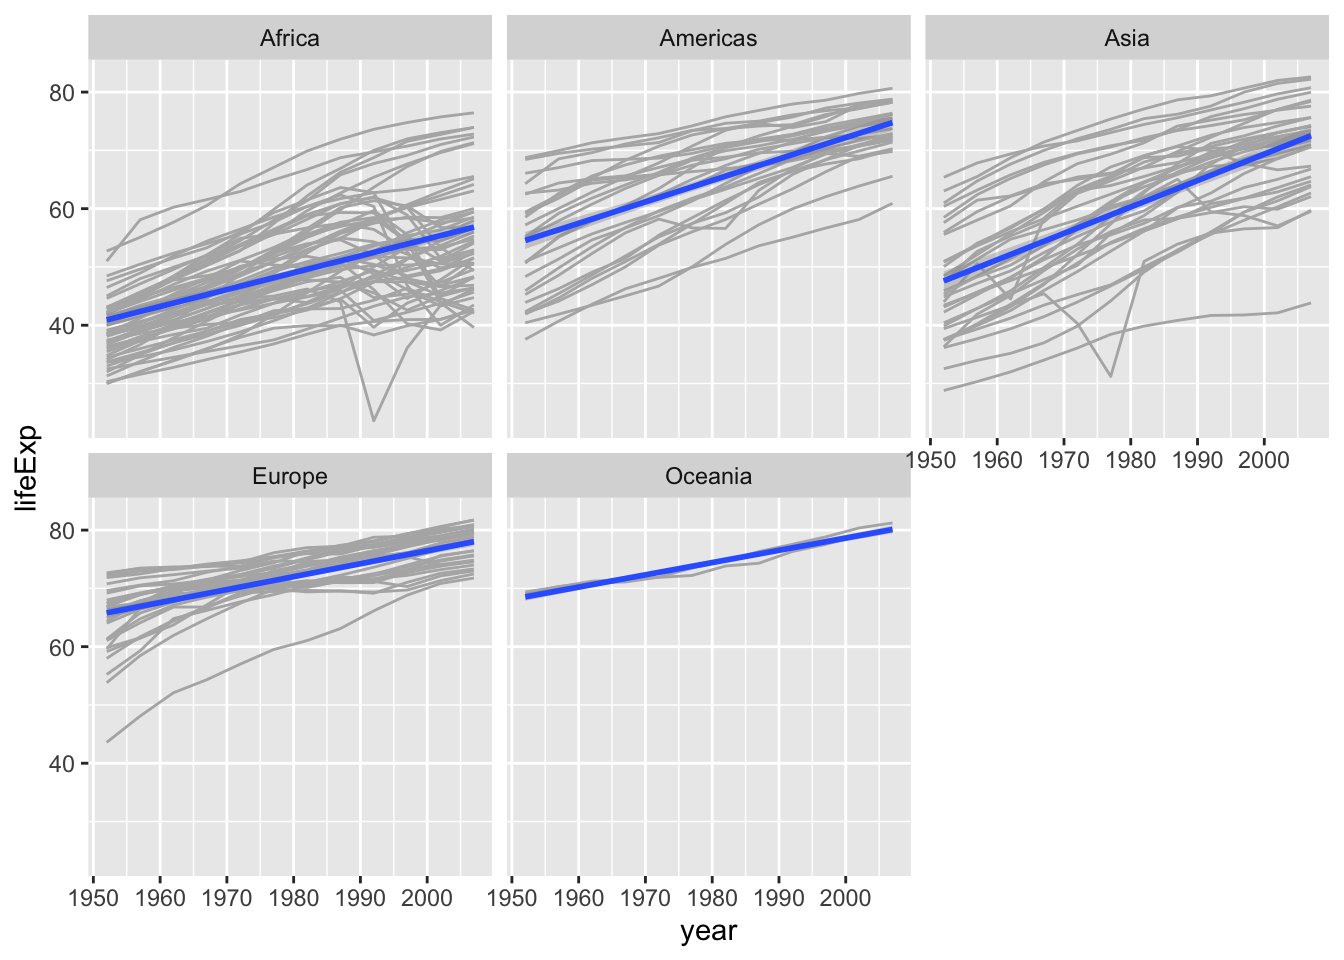
\includegraphics[scale=0.3]{practica2-img-gapminder-lifeExp.png}
\end{center}

\item (de ac\'a en adelante, trabajar con el dataset penguins del paquete palmerpenguins). ?`Cu\'antas filas y columnas hay en el dataset penguins?

\item  Dar una estad\'istica descriptiva de la variable \lstinline{bill_depth_mm}.

\item Hacer un \lstinline{scatterplot} de \lstinline{bill_depth_mm} (en el eje $y$) vs. \lstinline{bill_length_mm} (en el eje $x$).

\item ?`Cu\'al ser\'ia un buen geom para ver la relaci\'on entre \lstinline{species} y \lstinline{bill_depth_mm}?

\item Corregir el siguiente c\'odigo:
\begin{lstlisting}
ggplot(data = penguins) +
  geom_point()
\end{lstlisting}

\item ?`Qu\'e significa el argumento \lstinline{na.rm} en \lstinline{geom_point()}? Usando el dataset de \lstinline{palmerpenguins} crear un gr\'afico donde se requiera usar ese argumento como \lstinline{TRUE}.

\item Agregar un ``caption'' al gr\'afico de arriba. Ayuda: Mirar la documentaci\'on de \lstinline{labs()}.

\item Recrear la siguiente visualizaci\'on. ?`A qu\'e aes deber\'ia mapearse \lstinline{bill_depth_mm}? ?`El mapeo debe ser global o local?
\begin{center}
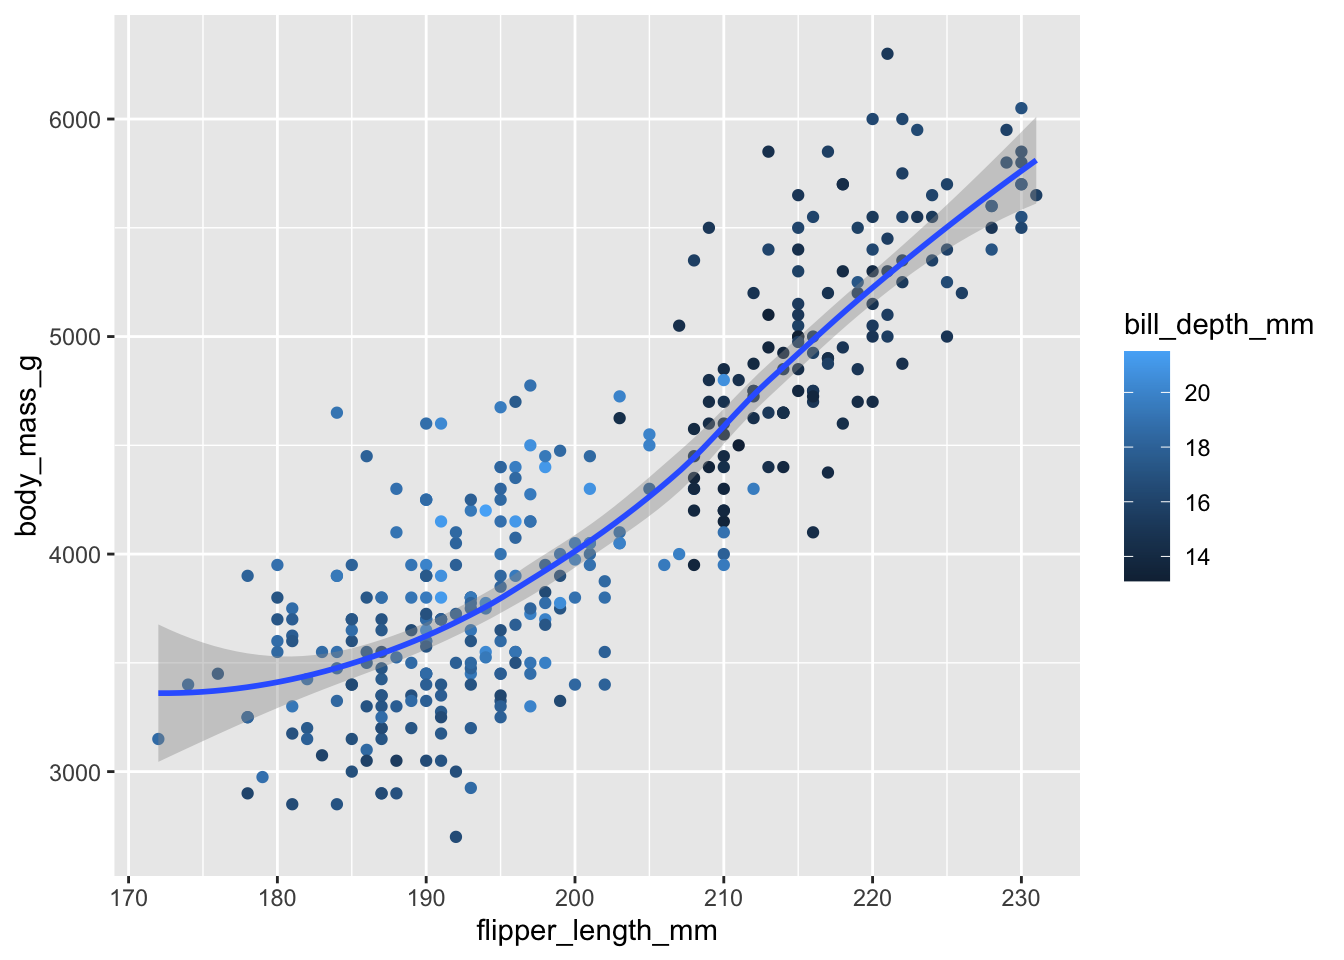
\includegraphics[scale=0.3]{practica2-img-penguins-mass.png}
\end{center}

\item Sin correr el c\'odigo, predecir qu\'e gr\'afico produce.
\begin{lstlisting}
ggplot(data = penguins,
       mapping = aes(x = flipper_length_mm, y = body_mass_g, color = island) ) +
  geom_point() +
  geom_smooth(se = FALSE)
\end{lstlisting}

\item Sin correr el c\'odigo, ?`estos dos gr\'aficos van a ser iguales o diferentes? ?`Por qu\'e?
\begin{lstlisting}
# grafico 1
ggplot(
  data = penguins,
  mapping = aes(x = flipper_length_mm, y = body_mass_g)
) +
  geom_point() +
  geom_smooth()

# grafico 2
ggplot() +
  geom_point(
    data = penguins,
    mapping = aes(x = flipper_length_mm, y = body_mass_g)
  ) +
  geom_smooth(
    data = penguins,
    mapping = aes(x = flipper_length_mm, y = body_mass_g)
  )
\end{lstlisting}

\item Sin correr el c\'odigo, predecir qu\'e gr\'afico produce.
\begin{lstlisting}
ggplot(data = penguins,
       mapping = aes(x = flipper_length_mm, y = body_mass_g, color = island) ) +
  geom_point() +
  geom_smooth(se = FALSE)
\end{lstlisting}

\item Sin correr el c\'odigo, ?`estos dos gr\'aficos van a ser iguales o diferentes? ?`Por qu\'e?
\begin{lstlisting}
# grafico 1
ggplot(
  data = penguins,
  mapping = aes(x = flipper_length_mm, y = body_mass_g)
) +
  geom_point() +
  geom_smooth()

# grafico 2
ggplot() +
  geom_point(
    data = penguins,
    mapping = aes(x = flipper_length_mm, y = body_mass_g)
  ) +
  geom_smooth(
    data = penguins,
    mapping = aes(x = flipper_length_mm, y = body_mass_g)
  )
\end{lstlisting}

\end{enumerate}

\end{document}


FACTORES


%%\item Las variables de clase "factor" (factores, o fct) son una clase especial que tiene R para trabajar con variables categ\'oricas. Una vez que se crean, los factores s\'olo pueden contener un conjunto pre-definido de valores que se conocen como los niveles del factor. ?`Qu\'e variables del dataset de gapminder son factores?
%
%\item Redefinir niveles. Supongamos que queremos cambiar la denominaci\'on del continente de Argentina a ``America'' (sin la s final). Prueben lo siguiente. ?`Qu\'e pas\'o? ?`Por qu\'e no funciona?
%\begin{lstlisting}
%class(gm.sur$continent)
%gm.sur$continent <- "America"
%class(gm.sur$continent)
%\end{lstlisting}
%
%Ahora prueben esto. ?`Entienden por qu\'e funciona?
%
%levels(gm.sur$continent) <- c("Africa", "America", "Asia", "Europe", "Oceania")
%class(gm.sur$continent)
%head(gm.sur)
%
%\item  Vamos a usar mucho "factores" a lo largo del curso, pero para que se den una idea, por ejemplo, los factores son muy \'utiles para codificar variables categ\'oricas en gr\'aficos. Vamos a ver esto bastante a lo largo de las clases, pero para que vean una aplicaci\'on simple, corran estas l\'ineas usando el paquete (que vamos a ver en las pr\'oximas clases) ggplot2.
%
%library(ggplot2)
%
%ggplot(data = gm.sur,
%       mapping = aes(x = year, y = pop, col = country)) +
%  geom_point(size = 3) +
%  theme_classic()
%
%Ahora corran lo siguiente. ?`En qu\'e difiere del anterior? ?`Pueden intuir por qu\'e tenemos ese resultado?
%
%ggplot(data = gm.sur,
%       mapping = aes(x = year, y = pop, size = country)) +
%  geom_point() +
%  theme_classic()
%
%?`Y si reemplazan size por shape dentro de aes(...)?
%
%4.13. Cambien m\'as cosas del c\'odigo anterior y prueben el resultado. De hecho, cambiar cosas y ver qu\'e pasa es una gran forma de aprender.

